\chapter{区块链云化框架调研分析}

本章首先通过快速评审获得Kubernetes operator赋能质量属性的策略集,  随后阐述区块链云化框架的设计原则, 最后结合区块链去中心化等特性以及设计原则分析筛选策略集形成基于Hyperledger Fabric的区块链云化框架的核心具体实施方案。

\section{快速评审}\label{section: rapid_reviews}

软件工程中, 快速评审(Rapid reviews)是一种轻量级的二级研究, 以实践为导向专注于及时的向研究人员提供证据\cite{cartaxo2020rapid}。本文对已发表的学术文章进行快速评审, 快速评审的目的是为了在较短时间内了解目前学术界使用Kubernetes operator进行云化的现状, 以及如何使用Kubernetes对现有系统进行赋能。随后, 对应文献对快速评审所得到的结果进行整理归纳得到Kubernetes operator如何为质量属性赋能的策略集。

本文的快速评审过程分为以下步骤: 首先进行自动化的全文数据库检索, 再筛选出与Kubernetes operator及架构改造强相关的文献, 接下来提取出本文所关注的质量属性及相关策略, 最后归纳整理出策略集。

{\footnotesize
\begin{longtable}[h]{m{60pt} m{210pt} m{40pt}<{\centering}}
    \caption[每个全文数据库的搜索字符串]{每个全文数据库的搜索字符串} \label{search_string} \\
        \toprule  
        \textbf{全文数据库}&\textbf{搜索字符串}&\textbf{文献数}\\
        \hline
        IEEE Xplore &(“kubernetes AND operator”) OR (“k8s AND operator”) OR (“custom resource defination”) & 23 \\

        ACM & “kubernetes operator” OR “k8s operator” & 7 \\

        Springer &((“kubernetes AND operator”) OR (“k8s AND operator”))AND ((“custom resource defination”) OR "CRD") & 0 \\

        ScienceDirect &(“kubernetes AND operator”) OR (“k8s AND operator”) OR (“custom resource defination”) & 0 \\
        \hline
        Scoups\&Google &“kubernetes operator”& 21(去重) \\
        \bottomrule
    \end{longtable}
}

如表\ref{search_string}所示, 为全面获取学术届对基于Kubernetes operator云化的策略, 确定了本次检索的全文数据库以及搜索字符串。本次检索主要针对计算机与软件工程领域的全文数据库\cite{lisboa2010systematic}(包含ACM、IEEE Xplore、Springer、ScienceDirect), 同时检索Scoups以及谷歌学术进行补充。最终, 围绕“kubernetes operator”为检索主题得到的共51篇论文。在文献筛选阶段, 本文根据筛选标准筛选出15篇与Kubernetes operator云化强相关的文献, 入选文献如表\ref{rapid_reviews}所示。文献筛选标准主要有:

\begin{itemize}[itemindent=2em]
    \item 论文的主要目的是利用Kubernetes对原有系统进行云化;

    \item 论文针对于Kubernetes operator方法;

    \item 论文介绍了具体的改造策略及相关的质量属性。
\end{itemize}

{\footnotesize
\begin{longtable}[h]{m{40pt} m{280pt} m{40pt}<{\centering}}
    \caption[快速评审入选文献列表]{快速评审入选文献列表} \label{rapid_reviews} \\
        \toprule  
        \textbf{文献编号}&\textbf{文献标题}&\textbf{文献引用}\\
        \hline
        [P1]&Enhancement of observability using Kubernetes operator&\cite{Shenoy2022496}\\
        
        [P2]&Designing a Kubernetes Operator for Machine Learning Applications&\cite{kanso2021designing}\\
        
        [P3]&Container orchestration on HPC systems through Kubernetes&\cite{zhou2021container}\\
        
        [P4]&Validation and Benchmarking of CNFs in OSM for pure Cloud Native applications in 5G and beyond&\cite{pino2021validation}\\
        
        [P5]&On-the-fly fusion of remotely-sensed big data using an elastic computing paradigm with a containerized spark engine on kubernetes&\cite{huang2021fly}\\
        
        [P6]&A Role-Based Orchestration Approach for Cloud Applications&\cite{yue2021role}\\
        
        [P7]&A Design of MANO System for Cloud Native Infrastructure&\cite{lee2021design}\\
        
        [P8]&Dynamic Updates of Virtual PLCs Deployed as Kubernetes Microservices&\cite{koziolek2021dynamic}\\

        [P9]&Suture: Stitching safety onto kubernetes operators&\cite{mahajan2020suture}\\
        
        [P10]&Automation of virtualized 5G infrastructure using mosaic 5G operator over kubernetes supporting network slicing&\cite{wiranata2020automation}\\
        
        [P11]&5G Cloud-Native: Network Management \& Automation&\cite{arouk20205g}\\
        
        [P12]&Proposed model for distributed storage automation system using kubernetes operators&\cite{sharma2020proposed}\\
      
        [P13]&Monitoring Resilience in a Rook-managed Containerized Cloud Storage System&\cite{baumann2019monitoring}\\
        
        [P14]&Reproducible Benchmarking of Cloud-Native Applications With the Kubernetes Operator Pattern&\cite{henning2021reproducible}\\
        
        [P15]&Pivotal Greenplum©for Kubernetes: Demonstration of Managing Greenplum Database on Kubernetes&\cite{patel2019pivotal}\\
        \bottomrule
    \end{longtable}
}

在数据提取阶段, 本文对5个提取项(文献标题、文献发表年份、质量属性、策略、所属领域)进行抽取, 共得到44条针对不同质量属性的相关策略。在数据归纳阶段, 由于不同的文献中对语义相同的质量属性用词存在明显差异, 本文根据国际软件质量评价标准ISO/IEC 25010:2011\footnotemark[1]\footnotetext[1]{\href{https://www.iso.org/standard/35733.html}{ISO/IEC 25010:2011 System and software quality models}}所定义的质量模型对收集到的文献中表述的质量属性进行映射, 同时对相同或相似的策略进行整理合并, 得到策略集如表所示。

{\footnotesize
\begin{longtable}[h]{m{40pt}|m{40pt}|m{20pt}|m{150pt}|m{80pt}}
    \caption[基于Kubernetes operator云化策略集]{基于Kubernetes operator云化策略集} \label{policy_set} \\  
        \hline
        \textbf{文献中质量属性}&\textbf{ISO质量属性}&\textbf{编号}&\textbf{策略}&\textbf{参考文献}\\
        \hline
        \multirow{4}*{\parbox[c]{40pt}{生产效率 \\ 效率}} & \multirow{4}*{易用性}
        &S1&容器化及Kubernetes能力 & [P3] \\\cline{3-5}
        & &S2&自动化配置复杂领域知识 & [P1, P2, P12-15] \\\cline{3-5}
        & &S3&自动化构建、部署应用程序 & [P6, P10, P11] \\\cline{3-5}
        & &S4&operator与helm结合 & [P1, P4, P13] \\\cline{3-5}

        \hline
        可迁移性 & 适应性
        &S1&容器化及Kubernetes能力 & [P1-P3, P8, P10-P12] \\\cline{3-5}

        \hline
        \multirow{2}*{可用性} & \multirow{2}*{可靠性}
        &S1&容器化及Kubernetes能力 & [P2, P15] \\\cline{3-5}
        & &S5&主备切换 & [P15] \\\cline{3-5}

        \hline
        \multirow{3}*{\parbox[c]{40pt}{可扩展性 \\ 可伸缩性 \\ 灵活性}} & \multirow{3}*{无}
        &S1&容器化及Kubernetes能力 & [P2, P3, P5, P7, P12, P15] \\\cline{3-5}
        & &S6&基于监控指标并进行伸缩处理 & [P2, P6, P13] \\\cline{3-5}
        & &S7&链外利用存储即服务 & [P15] \\\cline{3-5}

        \hline
        \multirow{4}*{安全性} & \multirow{4}*{安全性}
        &S8&RBAC & [P2] \\\cline{3-5}
        & &S9&自定义访问控制机制 & [P9] \\\cline{3-5}
        & &S10&多用户认证授权机制 & [P3, P13] \\\cline{3-5}
        & &S11&资源隔离 & [P13] \\\cline{3-5}

        \hline
        \multirow{1}*{可监控性} & \multirow{1}*{无}
        &S12&基于Prometheus的监控体系 & [P1, P5, P12, P13] \\\cline{3-5}
        \hline
    \end{longtable} 
}

\section{设计原则}\label{section: framework_characteristics}

区块链云化框架致力于在BaaS一站式构建、管理、托管和运维区块链网络及其应用的基础上更深入云原生底层基础设施Kubernetes的底层, 有效利用云能力对Fabric基础设施赋能, 需要满足以下原则:

\begin{itemize}[itemindent=2em]
    \item 易用性: 在Kubernetes上启动管理Hyperledger Fabric网络并部署链码需要专业的领域知识, Fabric各组件的配置项繁多且与Kubernetes适配极易出错。区块链云化框架需屏蔽底层Fabric配置与Kubernetes逻辑, 帮助用户采用命令行配置的方式提供完整的Fabric各组件的全生命周期管理;

    \item 可迁移性: 区块链云化框架需要具备基础架构的云独立性, 本框架依托Kubernetes, 可以方便的迁移到支持Kubernetes的任何云;

    \item 可视运维: 当前区块链系统缺乏一套涵盖不同层面的标准方法来监控区块链及其智能合约的运行\cite{zhangfuli2021smartcontract}。 区块链云化框架需提供基本运维能力, 有效复用云上监控方案为区块链系统提供7*24小时可视化资源监控能力;

    \item 安全性: 区块链云化框架需要具备有效的认证、鉴权、准入机制来确保区块链系统的安全性; 具备可插拔的共识算法取保区块链的去中心化、可追溯等特点, 支持完善的用户密钥授权、保存、隔离处理以及提供可靠的故障恢复能力;

    \item 可扩展性: 区块链云化框架需按照模块化配置, 将Kubernetes底层的计算资源、存储资源、网络资源等供给Fabric, Fabric的Ca、Peer、Orderer基本组件的证书认证、共识、TLS加密、存储等功能模块作为可配置项进行命令式配置; 该框架能够确保系统核心底层逻辑稳定运行的同时, 对外提供小而精的扩展边界, 实现系统的高内聚与低耦合;

    \item 透明性: 区块链云化框架需保证区块链上所有的交易记录是可追溯的、不可篡改的, 区块链交易过程以及获取交易产生的记录需要专业人员才能获取操作, 非专业人员难以理解, 框架需通过简单透明的方式获取交易记录。
\end{itemize}

\section{策略集应用}\label{section: policy_set_application}

通过快速评审的方式形成的基于Kubernetes operator云化策略集作为可选指导方案, 需要贴合区块链领域自身约束才能有效纳入区块链云化框架中落地。本节将围“所选策略为何能提升质量属性”以及“所选策略是否适用于Fabric”进行阐述。

容器化在云原生应用程序中的拥有更高的部署效率\cite{zhou2021container}、可迁移性。容器化可以使每个软件应用程序在隔离的环境中运行, 其将应用程序及其库、配置文件和其他依赖项封装在一起, 确保了环境兼容性, 从而使用户能够轻松地在不同的环境中移动和部署程序。因此, 容器化使得应用程序具备极强的可迁移性。Docker\footnotemark[1]\footnotetext[1]{\href{https://www.docker.com/}{Docker官网}}是容器化的典型代表, 其可以将运行态的容器打包成镜像(image)并储存在在线存储仓库中。Docker容器不是虚拟机, 这意味着它可以使用宿主机现有的网络接口\cite{shah2019building}。一旦创建了容器, 就可以为容器提供一个专用环回接口, 用于内部通信, 完成部署。

Kubernetes作为容器管理调度平台, 其具备强大的调度、伸缩和自恢复能力。Kubernetes会自动打包应用程序, 并根据预设需求运行Pod并管理容器。利用自身机制, Kubernetes可以轻松的将Pod进行横向扩容(Horizontal Pod Autoscaler, 简称HPA)或纵向扩容(Vertical Pod Autoscaler, 简称VPA)。Kubernetes提供了强大的容器自恢复能力, 可以自动重启在执行过程中失败的容器, 并杀死那些没有响应用户定义的健康检查的容器。但如果节点本身死亡, 那么它会替换并重新安排发生故障的容器到其他可用节点上。

Hyperledger Fabric官方提供了Binaries和Docker镜像两种安装方式\footnotemark[1]\footnotetext[1]{\href{https://github.com/hyperledger/fabric/blob/main/scripts/bootstrap.sh}{fabric\_bootstrap.sh}}, 其天然的满足容器化构建。一旦Fabric以镜像的方式托管于Kubernetes, 即可原生的利用Kubernetes进行高可用的管理。

值得注意的是, 区块链网络是去中心化的网络, 所有的节点共同参与记账, 只需要网络中的大多数(超过51\%)节点的账本状态一致即可, 并不需要所有网络中的所有的节点时刻保持高可用状态。同时, 无论是基于Kubernetes的多副本伸缩还是基于监控指标进行伸缩仅保证的是无状态应用的高可用性, 并不解决数据一致性问题, 所以为某个Fabric节点增加多副本进行可伸缩意义不大, 利用Kubernetes的自恢复能力保证单Fabric节点可用即可。

Blockchain Automation Framework采用脚本方式将Fabric部署于Kubernetes, 仅仅成了一次性自动化构建、部署Fabric的任务。这虽然能在一定程度上提升Fabric网络的部署效率, 但这不仅无法将Fabric复杂的领域知识以插拔化的方式配置进入云基础设施内部而且与helm的弊端一样, 不能对已经部署完成的Fabric网络各节点进行完整软件生命周期管理。Kubernetes operator提供的CRD方式可以插拔式地领域知识注入进云基础设施内部, 降低了Kubernetes运维人员对Fabric网络的二次学习成本。通过operator与Fabric helm的结合不仅能够提升Fabric网络的部署效率, 也可以时刻监听helm状态实现对整个网络进行完整生命周期管理。

虽然针对Peer节点的可伸缩性意义不大, 但从海量数据存储的角度来看, 使用云存储是加强区块链网络存储一种替代方法, 它减少了因区块存储空间有限而造成的限制\cite{gai2020blockchain}。云可以为区块链网络提供提供存储即服务(Storage as a Service, 简称SaaS)作为一种可扩展的链外解决方案。Kubernetes的SaaS通过服务的形式精细化使用存储资源, 实现了对存储定义(PVC)和存储申请(StorageClass)的灵活分离。Fabric网络的世界状态是一种脱链的链外附加缓存机制, 其最终被保存在链外的LevelDB或CouchDB中。同时, 世界状态的丢失并不会对区块链中的数据产生影响。这种链外存储机制可以使得Fabric网络能够通过Kubernetes的SaaS机制挂载外部存储单元不必关心存储资源的实际物理位置, 能够做到存储资源的即插即用。 

安全性方面, 区块链领域频繁的出现安全问题可能会动摇人们对去中心化应用的信任, 访问控制是提供云数据安全和隐私的一种基本方法, 可以防止未经授权的用户侵入云数据。不可靠的访问控制方法也会影响其他功能, 如身份验证、授权和数据审核。除自定义访问控制机制外, 云中的传统访问控制方法主要基于成熟的访问控制策略, 现有的传统访问控制策略分为四种: 自主访问控制(Discretionary Access Control, 简称DAC)、强制访问控制(Mandatory Access Control, 简称MAC)、基于角色的访问控制(Role-Based Access Control, 简称RBAC)和基于属性的访问控制(Attribute-Based Access Control, 简称ABAC), 其对比如表\ref{access_control}所示。

{\footnotesize
\begin{longtable}[h]{m{20pt} m{200pt} m{60pt} m{60pt}}
    \caption[访问控制机制]{访问控制机制} \label{access_control} \\
        \toprule  
        \textbf{名称}&\textbf{机制}&\textbf{优点}&\textbf{缺点}\\
        \hline
        DAC & 根据被操作对象的权限控制列表或者权限控制矩阵决定用户的是否能对其进行操作 & 操作简单 & 权限控制分散, 不利于管理 \\

        MAC & 每个对象含有权限标识, 每个用户也含有权限标识, 用户能够操作对象取决于双方权限标识的关系 & 适合机密或等级严格的场景 & 缺乏灵活性 \\

        RBAC & 一个用户关联一个或多个角色, 一个角色关联一个或多个权限, 根据权限需要创建角色并与用户绑定 & 灵活易扩展、职责分离 & 未提供操作顺序控制机制 \\

        ABAC & 根据规则动态计算一个或一组属性是否满足某种规则并授权判断 & 集中管理、按需实现不同粒度权限控制 & 不直观、规则复杂过多会出现性能问题 \\
        \bottomrule
    \end{longtable}
}

云化框架需要在Kubernetes上部署管理Fabric网络, 需要限制Kubernetes上其他用户对Fabric网络节点运行时的权限。在DAC中, 合法用户(如云服务提供商)根据自主访问控制策略来允许其他用户(如云用户)访问操作对象\cite{lopez2018access}, 同时阻止非授权的用户访问。DAC操作简单, 云用户能够进行灵活的访问控制, 然而DAC不需要严格的规则造成了权限管理的过于分散, 不利于综合管理; MAC则解决了DAC权限控制过于分散的问题, MAC是通过预定义的信任策略实现且该策略不能动态更改, 目标是限制访问的用户对目标对象的操作能力, MAC过于强调保密性, 管理缺乏灵活性; ABAC将访问规则写在配置文件里以实现多粒度的权限控制, 但是由于定义权限时不易看出用户和对象间的关系, 很容易给集群管理者带来运维上的麻烦; RBAC基于角色的权限控制体系, 能够实现“以岗定人”的目标。 虽然RBAC没有提供顺序操作的控制机制, 但Fabric中Orderer节点的功能本质上就是对无序的交易进行排序,所以这并不影响Fabric网络的正常交易流程。

云化框架除启用Kubernetes RBAC的授权机制外, 需要搭配命名空间(Namespace)进行资源隔离。并且应当在命名空间层面提供RBAC而不是集群。使用命名空间来隔离工作负载是一项基本的安全最佳实践, 云化框架可以主动使用命名空间所提供的分割功能可以将Fabric网络隔离在单独的命名空间内, 形成逻辑上的小组, 这可以实现与其他工作负载进行资源与安全性的隔离。

上述安全策略只是保护Fabric网络的第一道防线, 防止非法操作Fabric网络各节点, 而不是作为一项保护Fabric网络内部交易流程以及数据篡改的的策略。由于Fabric网络是基于MSP的认证性网络, 所以Fabric网络的参与者需要提供可认证的身份信息, 即Fabric网络含有多用户认证授权的机制。然而, 手动生成的Fabric网络密钥以文件的形式保存, 增加了密钥泄漏的风险, 云化框架需要结合Fabric的多用户授权机制提供安全的证书管理策略。

Prometheus\cite{sukhija2019towards}作为云原生领域的监控事实标准, 其是一个时序数据库又是一个监控系统, 有着强大的功能和良好的生态。
Grafana可以与各种其他类似于Prometheus的数据源进行交互并进行可视化。基于Prometheus的监控体系可以
收集开放的监控指标并进行多维度数据模型的灵活查询, 极大的增强了被监测系统的的可监控性。Fabric网络各节点的运行终态是Pod, 利用Prometheus监控体系可以无侵入式的收集Fabric网络各节点的监控指标, 并将指标数据以Grafana图表的方式展示, 真正做到7*24小时可视运维。

Fabric致力于构建透明、公开、去中心化的企业级分布式应用, 区块链云化框架需要在以下方面满足透明性原则。首先, 区块链云化框架构建Fabric网络过程的透明性, 区块链云化框架需要具备完备的日志体系, 日志能够提供记录区块链云化框架操作Fabric网络的行为以及Fabric网络的状态, 并能够规范的表达出来; 其次, 对于链上交易而言, Fabric网络本就是公开透明的。 区块链云化框架不能屏蔽这一特性, 需要对Fabric网络账本具备更加简易、公开、透明的命令式查询渠道, 如命令式查询交易记录。

综上, 如表\ref{policy_set_application}所示, 在区块链Fabric网络场景下结合快速评审的结果以及云化框架应当满足的设计原则, 剔除了3条不适用于Fabric去中心化网络特点的策略(S5、S6、S9), 最终形成了基于Hyperledger Fabric的区块链云化框架的9个核心策略实施方案。

\begin{figure}[h] %figure环境,h默认参数是可以浮动,不是固定在当前位置。如果要不浮动,你就可以使用大写float宏包的H参数,固定图片在当前位置,禁止浮动。
    \centering %使图片居中显示
    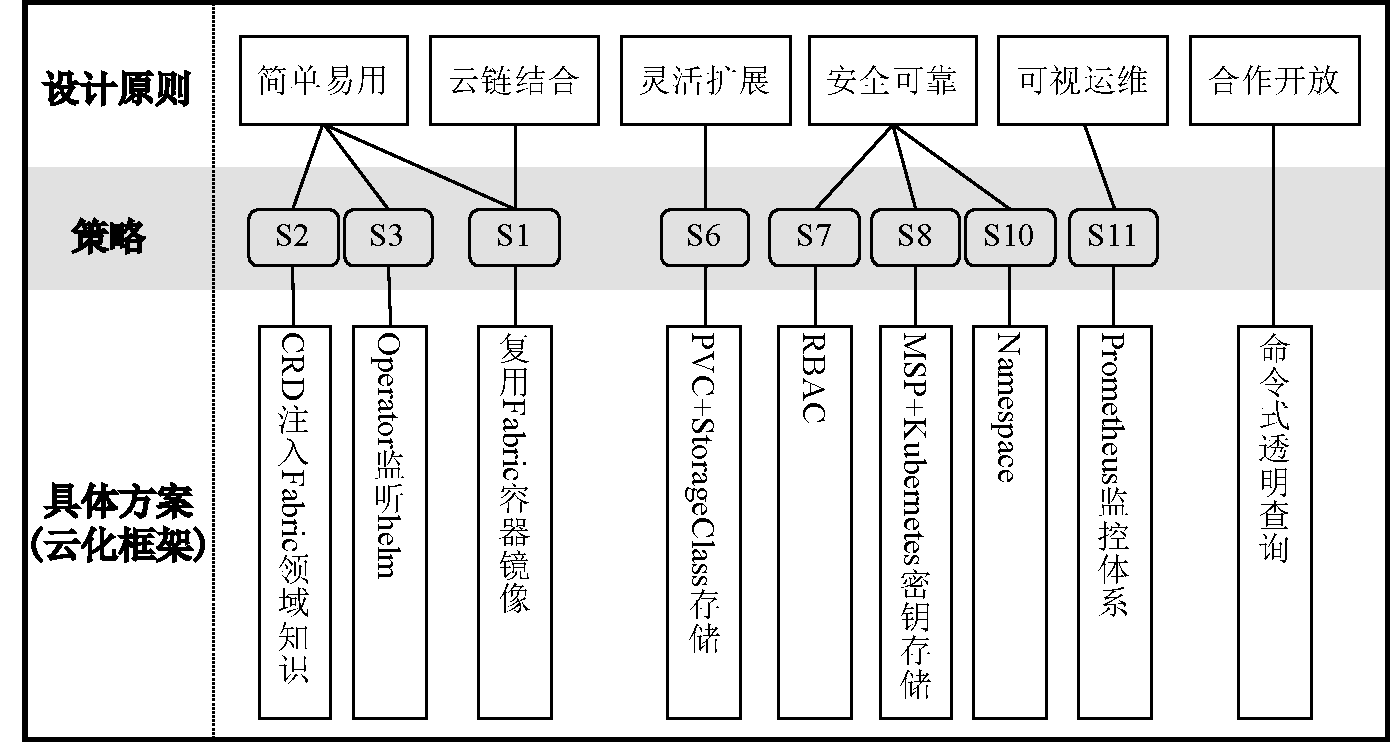
\includegraphics[width=1.0\textwidth]{FIGs/chapter3/policy_characteristics.pdf} %中括号中的参数是设置图片充满文档的大小,你也可以使用小数来缩小图片的尺寸。
    \caption{策略集应用} %caption是用来给图片加上图题的
    \label{policy_set_application} %这是添加标签,方便在文章中引用图片。
\end{figure}%figure环境


\section{本章小结}

本章为了解Kubernetes operator如何云化传统领域并对质量属性赋能, 首先详细介绍了快速评审的过程并得到基于Kubernetes operator云化策略集;其次, 本章重点介绍了基于Hyperledger Fabric的区块链云化框架所应满足的6条设计原则; 最后结合Fabric网络特性以及区块链云化框架设计原则对上述策略集进行筛选, 形成了基于Hyperledger Fabric的区块链云化框架的9个核心策略实施方案。